\section{Potenziali con orbite chiuse e limitate}

\begin{frame}{Potenziali centrali con orbite limitate}

\begin{block}{Teorema di Bertrand}

among central force potentials with bound orbits, there are only two types of central force potentials where all bound orbits are also closed:

\begin{itemize}

\item Inverse square central force : $V(vec{r})=\frac{-k}{r}$

\item harmonic oscilaltor: $V(\vec{r})=\frac{1}{2}kr^2$

\end{itemize}

\end{block}

\end{frame}

\begin{wordonframe}{potenziale che ammette orbite chiuse}

Punto stazionario di V ( cio\'e del potenziale efficacie).

Stabilit\'a orbita: $\TtwoDy{r}{V}<0$

\end{wordonframe}

\section{Orbite Kepleriane}

\begin{frame}{Problema ridotto}

\begin{columns}

\begin{column}{0.3\textwidth}

\input{reducedproblem}

\begin{align*}
&m_1\ddvec{r}_1=\frac{m_1m_2G}{r^3}\vec{r}\\
&m_2\ddvec{r}_2=\frac{m_1m_2G}{r^3}\vec{r}\\
&\mu\ddvec{r}=-k^2\frac{\vec{r}}{r^3}=-\frac{\gamma}{\mu}\frac{\vec{r}}{r^3}
\end{align*}


\end{column}

\begin{column}{0.7\textwidth}

\begin{block}{Costanti del moto}

\begin{align*}
&E_T=\frac{1}{2}m_1\dvec{r}_1^2+\frac{1}{2}m_2\dvec{r}_2^2-G\frac{m_1m_2}{r}\\
&=E_{CM}+E=\frac{1}{2}M\dvec{R}^2+\frac{1}{2}\mu\dvec{r}^2-G\frac{M\mu}{r}
\end{align*}

\begin{align*}
&\vec{J}=\mu\vec{r}\wedge\dvec{r}\\
&\vec{J}\cdot\vec{r}=0\\
&\vec{J}\cdot\dvec{r}=0
\end{align*}

\begin{align*}
&\vec{L}=\dvec{r}\wedge\vec{J}-\gamma\frac{\vec{r}}{r}=\dvec{r}\wedge\vec{J}-Gm_1m_2\frac{\vec{r}}{r}\\
&\dvec{L}=0\\
&\scap{J}{L}=0\\
&\scap{L}{r}=\frac{1}{\mu}J^2-\gamma r\\
&L^2=\gamma^2+\frac{2}{\mu}EJ^2
\end{align*}

\end{block}

\end{column}

\end{columns}

\end{frame}

\begin{wordonframe}{Definizione problema 2 corpi attrazione newtoniana}

\begin{align*}
&\vec{R}=\frac{m_1\vec{r}_1+m_2\vec{r}_2}{M}\\
&\vec{r}=\vec{r}_1-\vec{r}_2
\end{align*}

$\vec{r}$ ruota in piano perpendicolare a $\vec{J}$ e $\vec{L}$ \'e sul piano dell'orbita.

\end{wordonframe}


\begin{frame}{forma dell'orbita}

\begin{columns}

\begin{column}{0.4\textwidth}

\input{conservedvector}

\begin{block}{Periodo orbitale}

\begin{align*}
&JT=2\mu\pi ab\\
&T=2\pi\sqrt{\frac{a^3}{k^2}}
\end{align*}

\end{block}

\end{column}

\begin{column}{0.45\textwidth}

\begin{align*}
&Lr\cos{v}+\gamma r=\frac{1}{\mu}J^2\\
&r=\frac{p}{1+e\cos{v}}\\
&p=\frac{J^2}{\gamma\mu},\ e=\frac{L}{\gamma}
\end{align*}

\begin{block}{Orbite ellittiche}

\begin{align*}
&E<0,\ e<1\\
&r_{min}=\frac{p}{1+e},\ r_{max}=\frac{p}{1-e}\\
&a=\frac{1}{2}(r_{min}+r_{max})=\frac{p}{1-e^2}=-\frac{\gamma}{2E}\\
&J_{max}=\gamma\sqrt{\frac{\mu}{2|E|}}
\end{align*}

\end{block}

\end{column}

\end{columns}

\end{frame}

\begin{wordonframe}{Orbita kepleriana}

L'orbita \'e una conica con asse lungo $\vec{L}$, il modulo di L dipende da E e J

\begin{align*}
&e\gtreqless1\Leftrightarrow L\gtreqless\gamma\Leftrightarrow E\gtreqless0\\
&a=\frac{\gamma}{2|E|}\\
&b/a=\sqrt{1-e^2}
\end{align*}

connessione tra aspetti geometrici e dinamici: $a=-\frac{\gamma}{2E}$.

Per una certa energia E J non pu\'o superare quel valore per cui $a=b$.

\begin{align*}
&dS=\frac{1}{2}rr\dot{\theta}\,dt\\
&J=2\mu\TDy{t}{S}
\end{align*}

Terza legge di Keplero: $T\propto a\expy{\frac{3}{2}}$ (per pianeti maggiori sistema solare $\msun{}/m\approx\num{e-3}$)

moto medio $\frac{2\pi}{T}$: $n^2a^3=k^2$

\end{wordonframe}


\begin{frame}{Elementi orbitali}



%% document-wide tikz options and styles

\tikzset{%
  >=latex, % option for nice arrows
  inner sep=0pt,%
  outer sep=2pt,%
  mark coordinate/.style={inner sep=0pt,outer sep=0pt,minimum size=4pt,
  fill=black,circle},%
	sundot/.style={
	fill, color=yellow, circle, inner sep=3.5pt}
}


\begin{tikzpicture} % "THE GLOBE" showcase


    \def\R{1.5} % sphere radius
    \def\angEl{5} % elevation angle
    \def\angAz{105} % azimuth angle
    \def\angPhi{-40} % longitude of point P
    \def\angBeta{19} % latitude of point P

    \pgfmathsetmacro\H{\R*cos(\angEl)} % distance to north pole
    \tikzset{xyplane/.style={cm={cos(\angAz),sin(\angAz)*sin(\angEl),-sin(\angAz),
                                  cos(\angAz)*sin(\angEl),(0,-\H)}}}
    \LongitudePlane[xzplane]{\angEl}{\angAz}
    \LatitudePlane[equator]{\angEl}{0}

     \filldraw[ball color=white, fill opacity=1] (0,0) circle (\R);
    \draw (0,0) circle (\R);
    \coordinate (O) at (0,0);
    \coordinate[mark coordinate] (N) at (0,\H);
    \coordinate[mark coordinate] (S) at (0,-\H);
%		\coordinate (horizon) at (-30.0:\R);
%		\coordinate (equator) at (\H,0);


    \draw[->] (0,-\H-5) -- (0,\R+5) node[above] {}; %axis of rotation
%		\draw[->,rotate=-30.0] (0,-\H-5) -- (0,\R+5) node[above] {\bf{Zenith}}; %axis of rotation

    \path[xzplane] (\R,0) coordinate (XE);

%		\DrawLatitudeCircle[\R,color=blue]{0} % equator
%		\DrawLatitudeCircle[\R,rotate=23.5,color=red]{0}
%		\node[right,color=red] at (horizon) {\bf{Horizon}};
%		\node[above=9pt, right=-5pt, color=blue] at (equator) {\bf{Equator}};
%		\node[label={above right:\bf{Equator}}] at (equator) {};

		\path (N) node[align=left, above=1.5em, right] {\textbf{North}\\ \textbf{pole}} (N);
		\path (S) node[align=left, below=1.5em, right] {\textbf{South}\\ \textbf{pole}} (S);
%    \node[above=10pt, left=3pt] at (N) {\bf{North}};
%    \node[above=2pt, left=12pt] at (N) {\bf{pole}};

%    \node[below=5pt, right=4pt] at (S) {\bf{South}};
%    \node[below=14pt, right=4pt] at (S) {\bf{pole}};

    \def\R{6} % sphere radius
    \def\angEl{5} % elevation angle
    \def\angAz{105} % azimuth angle
    \def\angPhi{-40} % longitude of point P
    \def\angBeta{19} % latitude of point P

    \pgfmathsetmacro\H{\R*cos(\angEl)} % distance to north pole
    \tikzset{xyplane/.style={cm={cos(\angAz),sin(\angAz)*sin(\angEl),-sin(\angAz),
                                  cos(\angAz)*sin(\angEl),(0,-\H)}}}
    \LongitudePlane[xzplane]{\angEl}{\angAz}
    \LatitudePlane[equator]{\angEl}{0}

    \filldraw[ball color=white, fill opacity=0.3] (0,0) circle (\R);
    \draw (0,0) circle (\R);

    \coordinate (O) at (0,0);
    \coordinate[mark coordinate] (N) at (0,\H);
    \coordinate[mark coordinate] (S) at (0,-\H);
		\coordinate (Equator) at (\H,0);
		\coordinate (Ecliptic) at (23.5:\R);
    \path[xzplane] (\R,0) coordinate (XE);

		\draw[->,ultra thick] (0:\R) arc (0:23.5:\R);
		\coordinate (tilt) at (11.75:\R);
		\node[right=5pt] at (tilt) {$23.5^{\circ}$};
%		\coordinate (obslat) at (75:0.4*\R);
%		\node[above=5pt] at (obslat) {$30^{\circ}$};
		\DrawLatitudeCircleName[\R,color=blue]{0}{celeq} % equator
%		\draw 
		\DrawLatitudeCircleName[\R,rotate=23.5, color=orange]{0}{ecl} % ecliptic
		\node[right=0.5em, color=blue] at (Equator) {\textbf{Celestial equator}};
		\node[above=0.5em, right=0.5em, color=orange] at (Ecliptic) {\textbf{Ecliptic}};
		\path[name intersections={of= celeq and ecl,by={vereq}}];%, [label=above left:\textbf{Autumnal equinox}]b}}];
		\coordinate[mark coordinate] () at (vereq) {};
		\path (vereq) node[align=right, below=1.3em, right] {\textbf{Vernal equinox}\\ March 20th}
		(vereq);
		\coordinate[mark coordinate] (sumsol) at (23.5:\R);
		\path (sumsol) node[align=right, above=1.3em, left=1em] {\textbf{Summer solstice}\\ June
		21st} (sumsol);
		\coordinate[mark coordinate] (winsol) at (23.5+180:\R);
		\path (winsol) node[align=right, below=1.5em, right=0.5em] {\textbf{Winter solstice}\\
		December 21st} (winsol);
		\coordinate[mark coordinate] (auteq) at (100.5:0.09*\R);
		\path (auteq) node[align=right, above=1.3em, left=0.5em] {\textbf{Autumnal equinox}\\
		September 23rd} (auteq);
		\coordinate[sundot] (sun) at (15:0.5*\R);
		\draw[->,very thick] (sun) -- (18.4:0.7*\R);
		\node[above=1.0em,right=0.1em] at (vereq) {$\aries$};
		\node[below=1.0em] at (sun) {\textbf{The sun}};
%		\draw[->] (auteq) -- (120:0.3*\R);
%		\node[mark coordinate,align=center,below right] at (a) {Vernal \\ equinox};
%		\node[mark coordinate,label=above left:\textbf{Summer solstice}]
%		\node[mark coordinate] at (a) {};
%		\coordinate[mark coordinate] (a) at (intersection-2);
%		\node[label={above right:\bf{Celestial horizon}},color=red] at (Horizon) {};
%		\node[label={right:\bf{Celestial equator}},color=red] at (Equator) {};

%		\DrawLongitudeCircle[\R]{\angAz+15}{} % xzplane

    \node[above=7pt, left=5pt] at (N) {\bf{North celestial pole}};
    \node[below=8pt, right=5pt] at (S) {\bf{South celestial pole}};

\end{tikzpicture}

\end{frame}



\begin{wordonframe}{Elementi orbitali}

Piano ecclittica: piano orbita solare rif geocentrico: ''intersezione della sfera celestecon il piano su cui giace l'orbita terrestre

Linea dei nodi \'e intersezione tra piano orbita pianeta e piano eclittica, i \'e l'inclinazione del piano dell'orbita rispetto al piano dell'eclittica

L'angolo $\Omega$ identifica l'orientazione della linea dei nodi rispetto al punto $\gamma$ posizione del Sole all'equinozio di primavera; l'angolo $\omega$ identifica la direzione del semi-asse maggiore rispetto alla linea dei nodi; l'angolo $\nu$ identifica la posizione del pianeta sull'orbita.

\end{wordonframe}


\begin{frame}{Orbite Kepleriane - legge del moto.}

\begin{columns}

\begin{column}{0.4\textwidth}

\begin{figure}[!ht]

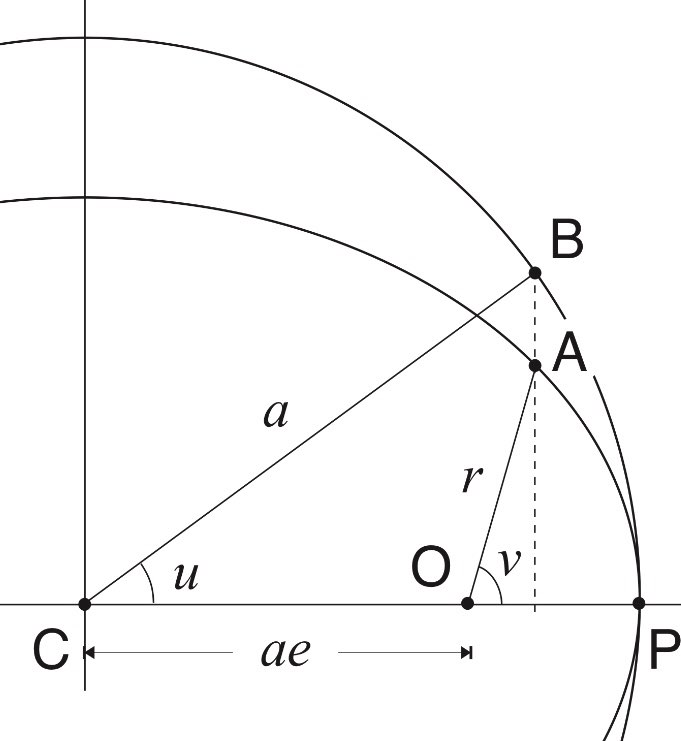
\includegraphics[width=\textwidth]{ellipseinO}

\end{figure}

\end{column}

\begin{column}{0.4\textwidth}

\end{column}

\end{columns}

\end{frame}

\begin{frame}{Approx. piccola eccentricit\'a}

\end{frame}

